\chapter{Decisiones operativas de marketing}

\section{Productos}

\section{Precios}

\subsection{Identificación de costos}

Identificamos los siguientes costos fijos:

\begin{itemize}
\item \textbf{S/. 256}: Servidores en la nube, Amazon EC2, máquinas del tipo t2.large (2 CPUs, 8GB RAM)
\item \textbf{S/. 600}: Alquiler de la oficina de desarrolladores
\item \textbf{S/. 150}: Recibos de luz y agua
\item \textbf{S/. 120}: Internet Claro de 8Mb
\item \textbf{3 x S/. 2000}: Salarios
\item \textbf{S/. 300}: Publicidad en redes sociales
\end{itemize}

No identificamos ningún costo variable.

\subsection{Política de precios}

Queremos brindar un servicio de calidad y fácil de usar. Pretendemos una penetración rápida y profunda en el mercado reduciendo el margen de ganancia al mínimo en un inicio, y luego incrementándolo una vez que los usuarios se acostumbren a la aplicación.

Tenemos dos frentes donde cobrar dinero. En primer lugar tenemos a los usuarios finales, a quienes se les ofrece un servicio de calidad por un precio razonable, no esperamos obtener ganancias de este grupo. De donde esperamos obtener ganancias es de cobrarle una comisión a los taxistas por cada encomienda que se les consiga. Durante los dos primeros meses que el taxista utilice la aplicación, gozará del 100\% de los beneficios de su trabajo, luego se le cobrará una comisión del 10\%. Esperamos que los taxistas ya familiarizados con la aplicación y conscientes de su beneficio, luego de dos meses de prueba gratis, estén dispuestos a pagar la comisión.

\section{Promoción}

\section{Distribución}

\section{Personas}

\section{Evidencia física}

\section{Procesos}

A continuación detallamos con diagramas de flujo los dos principales procesos de este proyecto. El primero es el registro de nuevos clientes y el segundo es el pedido de nuevas encomiendas; este último se expone desde los puntos de vista tanto del cliente como del taxista.

\begin{figure}[htb]
\centering
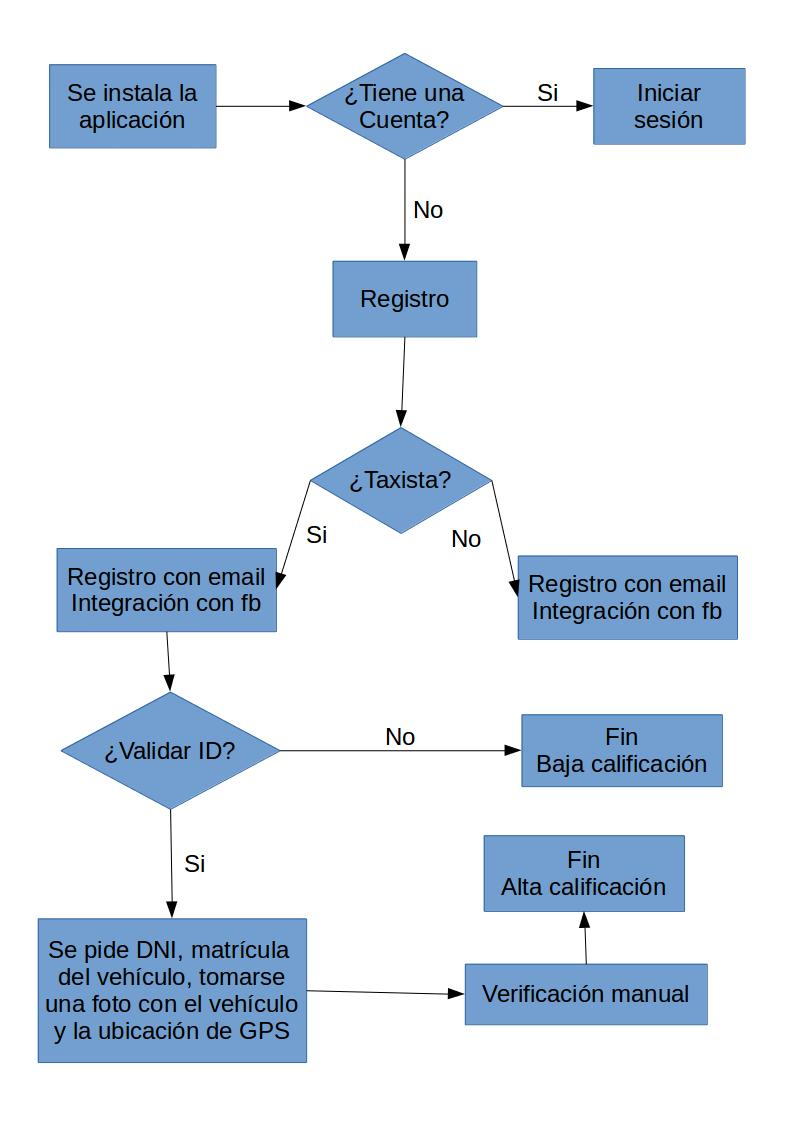
\includegraphics[width=0.8\textwidth]{./img/proceso_registro_nuevo_usuario.jpg}
\caption{Proceso de registro de un nuevo usuario} \label{fig:proc_nuevo_usuario}
\end{figure}

En la figura \ref{fig:proc_nuevo_usuario} vemos el proceso necesario para añadir un nuevo usuario al sistema, este puede ser un cliente o un taxista. En el caso de que sea un taxista, se pide un paso adicional: la verificación de identidad. Este paso es importante puesto que nos permite brindarle un servicio de calidad a los clientes, y tratamos de incentivarlo con un sistema de calificación, si te verificas obtienes una alta valoración, y si no lo haces tu valoración es muy baja, con lo que es menos probables que los usuarios te escojan a la hora de solicitar el servicio de courier. Pensamos realizar la verificación de forma manual, consultando la información del DNI y comparándola con la foto que nos envíe, lo mismo con el vehículo.


\begin{figure}[htb]
\centering
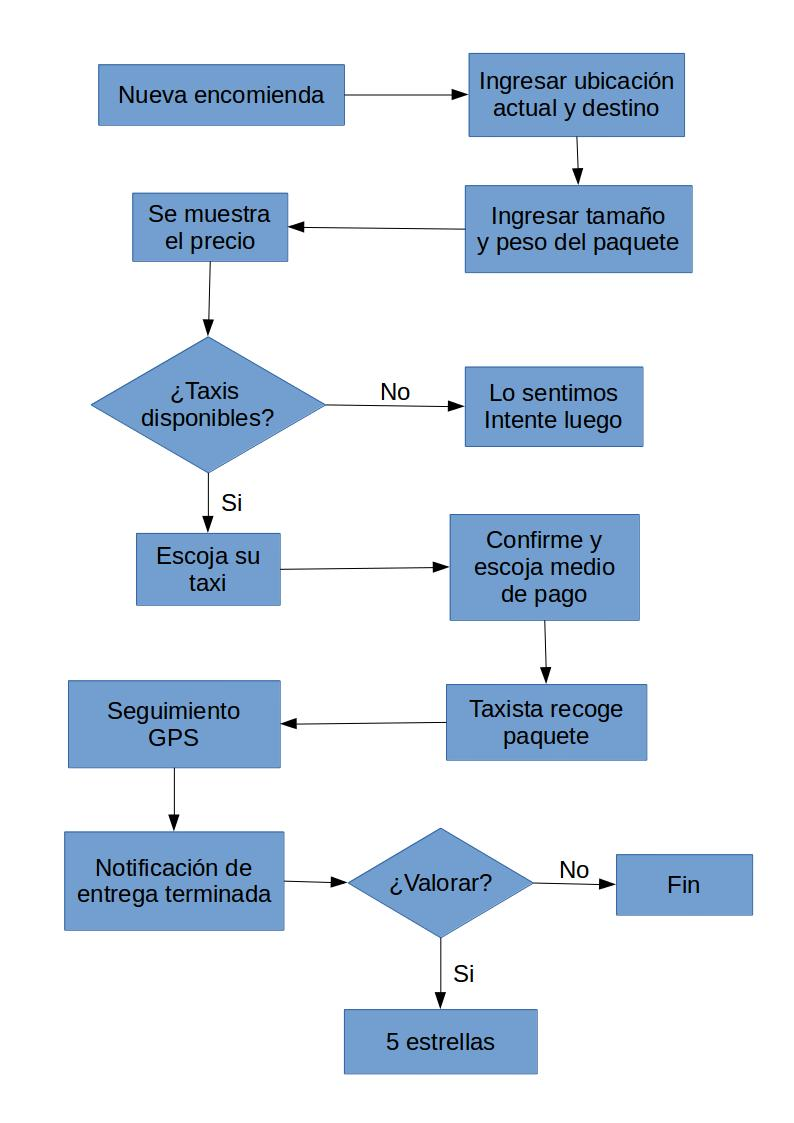
\includegraphics[width=0.8\textwidth]{./img/nueva_encomienda.jpg}
\caption{Proceso de solicitud de una nueva encomienda, desde el punto de vista del usuario final} \label{fig:proc_nueva_encomienda}
\end{figure}


\begin{figure}[htb]
\centering
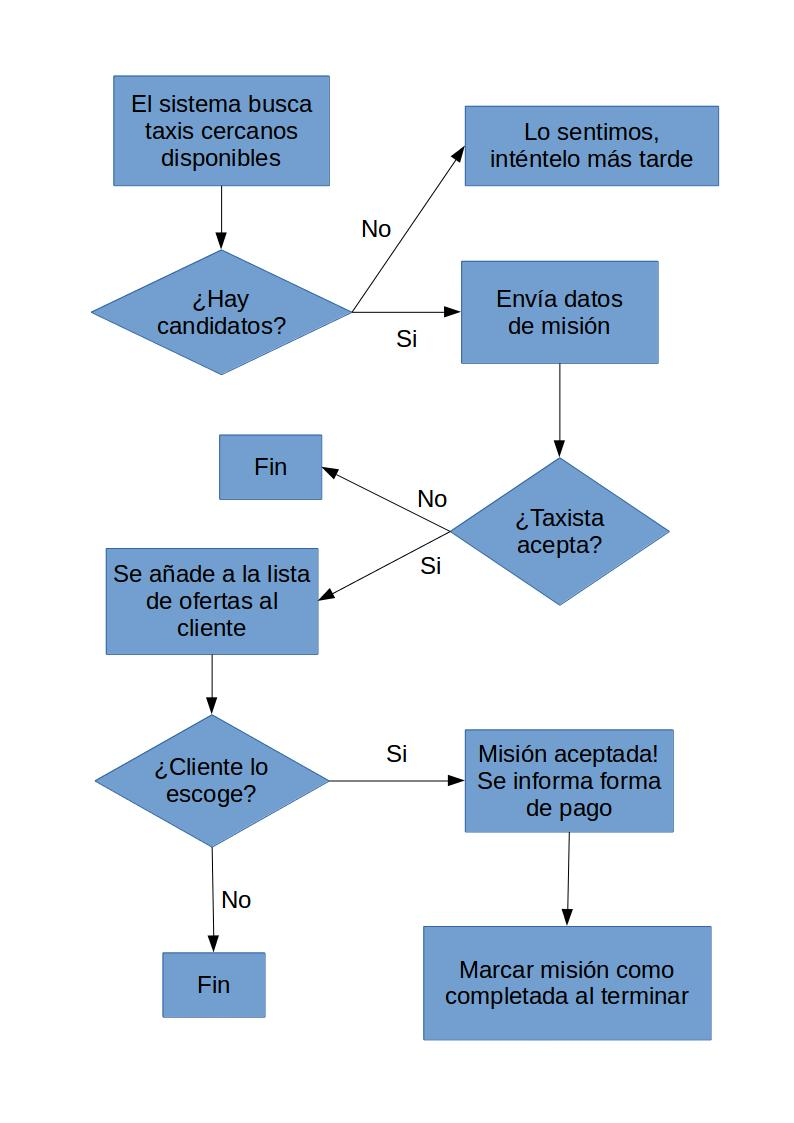
\includegraphics[width=0.8\textwidth]{./img/taxista.jpg}
\caption{Proceso de solicitud de una nueva encomienda, desde el punto de vista del taxista} \label{fig:proc_taxista}
\end{figure}


En la figuras \ref{fig:proc_nueva_encomienda} y \ref{fig:proc_taxista} se aprecia el proceso mediante el cual se solicita una nueva encomienda. El precio que se le muestra al cliente depende de la distancia del recorrido, así como del tamaño y peso del paquete. Este precio es calculado por nuestro sistema y no es negociable, de ese modo queremos crear una tarifa objetiva y estándar. Los usuarios finales obtienen una lista de taxistas que pueden cubrir el servicio, cada taxista con su respectiva valoración. Mientras el paquete se encuentra en el taxi, la aplicación hace un seguimiento GPS para que el cliente sepa donde se encuentra su paquete en todo momento. Una vez que el paquete llega a su destino, el cliente recibe una notificación y la opción para poder valorar el servicio del taxista. Puede llamar para ver si el paquete llego bien por ejemplo, y en base a eso calificar.

Los taxistas desde su punto de vista van recibiendo constantemente misiones de courier que pueden ir aceptando o ignorando. También es importante notar que al aceptar una misión, el taxista simplemente se añade a la lista de candidatos para el cliente, pero es en última instancia el cliente quien decide qué taxista realizará el servicio. Esta es otra forma de motivar que los taxistas tengan una buena calificación.